\section{Introduction}

Since the creation of Inductive Program Synthesis (IPS) in the 1970s~\cite{Kitzelmann2009}, researchers have been striving to create systems capable of generating programs competitively with human intelligence. Modern IPS methods often trace their roots to the fields of machine learning, logic programming, evolutionary computation and others.

Some IPS systems, such as MagicHaskeller, were created to be used as a teaching tool for people learning to program in the Haskell language. Other IPS systems have been used to perform Automated Program Repair~\cite{Perelman2014} to fix bugs in human written code.

As IPS systems become better at generating the same kinds of programs humans would generally write, there will likely be many more applications that have large impacts on the fields of machine learning, artificial intelligence, and software development.

The similarities and differences of IPS methods have been discussed~\cite{Kitzelmann2009}, but their performance is rarely compared on problem sets that could provide concrete insight into the capabilities and limitations of each method.

This is largely due to how recently many of current methods have been introduced. TerpreT and the Grammar Guided Genetic Programming system proposed in~\cite{Forstenlechner:2017:eurogp} have been published for less than a year. Flash Fill and Magic Haskeller were both introduced in the 2010s. PushGP, although first published in 2002, has improved greatly on IPS tasks in recent years~\cite{Helmuth2015a}.

A demonstrative problem set has been compiled that assess an IPS method's ability to work within a range of levels of abstraction~\cite{Gaunt2016}, manipulate a variety of data types, utilize complex control structures and produce an arbitrary number of outputs of various forms~\cite{Helmuth2015b}.

This investigation is exclusively considering each method's ability to find solutions. Other measures, such as runtime or hardware models, are not thoroughly examined. In order to determine if a method can find solutions to a problem, the problem must first be phrased in its entirety to the method. This is not always possible.

It should be noted that we have much more experience using genetic programming than Flash Fill, MagicHakseller, and TerpreT. We made a best effort to become as familiar as possible with all methods used in this comparison. There is still a chance that these systems can be used in ways we are unaware of that could change the results this experiment.

The conclusions drawn from this comparison will speak to the flexibility, and success rate, of each considered method when applied to general IPS tasks.

\section{Problems}

\subsection{Basic Execution Models Problems}

The first set of 8 problems, taken from \cite{Gaunt2016}, was designed to demonstrate TerpreT's ability to synthesis programs in a variety of execution models that span multiple levels of abstraction. These execution models are: Turing Machine, Boolean Circuits, Basic Block, and Assembly Language. As stated by \cite{Gaunt2016}, the problems in this set progress from more abstract execution models towards models which resemble assembly languages. These problems demonstrate how a system performs across a variety of low-level domains. 
The problems in this set are described below:


\begin{description}

\item[Invert] Given a binary string (binary tape), invert all the bits. 

\item[Prepend Zero] Insert a $0$ in the first index of a binary string and shift all other bits to the right.

\item[Binary Decrement] Given an input binary string equal to a positive decimal number, return a binary string equal to the input number decremented by one.

\item[2-bit Controlled Shift Register] Given input bit ($r_1$, $r_2$, $r_3$), return the same bits, except swap the order of $r_2$ and $r_1$ if $r_1 == 1$.

\item[Full Adder] Given a carry bit, $c_{in}$, and two argument bits, $a$ and $b$ , output a sum bit, $s$, and carry bit, $c_{out}$, such that  $s + 2c_{out} = c_{in} + a_1 + b_1$.

\item[2-bit Adder] Given input bits $a_1$, $a_2$, $b_1$, and $b_2$, output $s_1$, $s_2$, and $c_{out}$ such that  $s_1 + 2s_2 + 4c_{out} = a_1 + b_1 + 2(a_2 + b_2)$.

\item[Access] Given an input array, $V$, and a positive integer, $i$, return $V_i$. Assume $0 < i < |A|$.

\item[Decrement] Given an input array, $V$ return a new array, $U$ such that $U_i = V_i - 1$.

\end{description}

In Flash Fill, binary strings were implemented as strings of $1$s and $0$s in a single cell that was set to the type "Text". In all other systems, the binary strings were implemented using vectors of boolean values.

The TerpreT system was originally given between 5 and 16 input-output examples for each of these problems. PushGP, MagicHakeller, FlashFill were also given between 5 and 16 input-output examples for each problem, with certain edge cases manually included while other test cases were generated.


\subsection{General Program Synthesis Benchmark Suite}
The second set of problems used in this comparison was designed as a benchmark suite for general program synthesis \cite{Helmuth2015b}. The 29 problems here require the synthesis of programs with similar characteristics to programs that humans write. Each problem in this suite was taken from an introductory computer science textbook, and therefore emulates the type of programming expected of students who are learning to program. While these benchmarks were first used in genetic programming, they are designed to be usable in any inductive program synthesis system that supports the required data types.

The problems in this set include those that require a range of data types, including strings, integers, floats, characters, and vectors. Many of the problems require outputs to be printed in the style of standard output, and one problem requires multiple output values. Additionally, most of the problems require some level of control flow to solve, whether through iteration, recursion, conditional execution, or list-manipulating higher-order functions.

Where the Basic Execution Models problem set is designed to test a system's ability to perform in low-level domains (binary circuits, assembly language, etc), the General Program Synthesis Benchmark Suite tests the ability to perform higher-level tasks.

Since we do not have space to describe all 29 problems here, consdering the following example: the Replace Space with Newline problem. In this problem, the input is a string, and the program must complete two tasks: it must print the input string after replacing each space character with a newline, and it must then functionally return the number of non-whitespace characters in the input string. At minimum, this problem requires the consideration of strings, characters, and printing; a solution will also likely include some type of iteration or string processing. The other 28 problems are thoroughly described in the original suite \cite{Helmuth2015b}.

%\subsubsection{Number IO}
%\subsubsection{Small or Large}
%\subsubsection{For Loop Index}
%\subsubsection{Compare String Lengths}
%\subsubsection{Double Letters}
%\subsubsection{Collatz Numbers}
%\subsubsection{Replace Space with Newline}
%\subsubsection{String Differences}
%\subsubsection{Even Squares}
%\subsubsection{Wallis Pi}
%\subsubsection{String Lengths Backwards}
%\subsubsection{Last Index of Zero}
%\subsubsection{Vector Average}
%\subsubsection{Count Odds}
%\subsubsection{Mirror Image}
%\subsubsection{Super Anagrams}
%\subsubsection{Sum of Squares}
%\subsubsection{Vectors Summed}
%\subsubsection{X-Word Lines}
%\subsubsection{Pig Latin}
%\subsubsection{Negative To Zero}
%\subsubsection{Scrabble Score}
%\subsubsection{Word Stats}
%\subsubsection{Checksum}
%\subsubsection{Digits}
%\subsubsection{Grade}
%\subsubsection{Median}
%\subsubsection{Smallest}
%\subsubsection{Syllables}

\section{Current State of the Art}

Below are descriptions of the five inductive program synthesis techniques compared in our experiments.

\subsection{Flash Fill}

Flash Fill, recently added to Microsoft Excel, uses version-space algebras to perform program synthesis from examples on string manipulation tasks~\cite{Gulwani2011}. It was designed to help non-programmers perform repetitive tasks that would otherwise require them to write Excel macro programs. As such, it is able to quickly create simple programs for one-off repetitive tasks in spreadsheet applications for non-programmers~\cite{Gulwani:2012:SDM:2240236.2240260, harris2011spreadsheet, Singh:2012:LSS:2212351.2212356, singh2012synthesizing}. Building on the use of version-space algebras for programming by demonstration~\cite{lau2003programming}, Flash Fill assumes few example inputs and must make simplifying assumptions about the problem space. In particular, the domain-specific language used here is designed for small string manipulation tasks that an end-user may want to perform without knowing how to program them. Adapting the technique for new domains would require a different domain-specific language that is carefully crafted to meet problem requirements while restrictive enough to allow for quick searching. Each different domain-specific language would also require a new synthesis technique; it is unclear whether Flash Fill will even be able to tackle many general program synthesis problems.

To test Flash Fills performance with our problem set, an Excel spreadsheet with one column per input and one column for output was created for each problem. Each spreadsheet included training data, which had both the input columns and output column populated, and unseen testing data, which left the output column cells empty. Flash Fill is deterministic and analytic, thus it was only run once per problem on a single data set.

It is not possible to pose tasks to Flash Fill that required multiple outputs. This includes problems that require printing values in addition to returning an output. Asking Flash Fill to generate each output value in separate cell was considered, but this would be two separate tasks and would not be comparable to the other IPS methods.

\subsection{MagicHaskeller}

MagicHaskeller~\cite{katayama2010,Katayama05} synthesizes functional Haskell programs through an exhaustive search of programs with the correct type signatures. It uses a Monte-Carlo algorithm to remove semantically equivalent programs from the search space~\cite{Katayama2008}. More recently, it has also integrated an analytic component based on \textsc{Igor2}~\cite{kitzelmann2011two}, which allows it to synthesize a greater range of programs than can be found in reasonable time using exhaustive search~\cite{katayama2011magichaskeller}. Additionally, a web interface is available running a time-limited version of MagicHaskeller intended as a Haskell teaching tool for new programmers~\cite{katayama2013}. These implementations make great use of Haskell's functional instructions, and they perform well on problems that require list manipulations and structural changes. While MagicHaskeller performs very quickly on simple problems without too many examples, it has trouble with problems that require a large number of examples to illuminate the relevant edge cases. Additionally, it seems to have trouble with problems that require conditional control flow.

MagicHaskeller uses specifications in the form of a predicate consisting of example function calls and their desired outputs. To then synthesize a function, MagicHaskeller generates a stream of functions that have the same signature as the example function calls. Thus generated functions have the same number of inputs, the same input types, and the same output type.

Generated functions are tested against the input predicate, and a sample of passing functions are presented to the user. The user can then "Exemplify" the suggested solution functions to see how they would behave given a variety of other inputs. If the user cannot find an adequate solution function, more functions can be generated until the entire stream has been processed.

MagicHaskeller was originally applied to a set of problems that mainly dealt with list manipulation. These types of prolbems are represeted in the problem set used in this comparison as well, but are generally more complex than what MagicHaskeller was shown to solve in~\cite{katayama2013}.

For our experiments, we used the web hosted version of MagicHaskeller. When using the MagicHaskeller web service, all MagicHaskeller users share the same dynamic programming table used for memoization, and the users cannot select which functions are included when searching. Due to MagicHaskeller being hosted on the web, it is difficult to embed in other systems. One benefit of using the publicly hosted version of MagicHaskeller is that users can suggest new contributions to the dynamic programming table, which potentially improves the search space for all users upon the next update of the MagicHaskeller system. 

\begin{figure}
\begin{verbatim}
((f [1, 2, 3] == [0, 1, 2]) && (f [-1, 1] == [-2, 0]))  
\end{verbatim}
\caption{An example predicate that can be supplied to MagicHaskeller. This particular predicate produces a solution to the Decrement problem.}
\label{fig:MHpred}
\end{figure}

Figure \ref{fig:MHpred} shows an example input predicate. Notice that multiple nested predicates can be supplied. MagicHaskeller supports the common primitive data types such as: integers, floats, strings and characters. Vectors and tuples are also supported, witch greatly expands the number of problems that were able to be posed to MagicHaskeller.

MagicHaskeller only allows for the synthesis of functions that produce a single output value. In order to pose questions that require multiple outputs, MagicHaskeller was given predicates that specified a tuple as an output. For problems that specify that values should be printed in addition to the output value, it was considered sufficient if MagicHaskeller could synthesis a program that produced a single string containing all printed values (including whitespace and newline) as an element of its output tuple.

\subsection{TerpreT}

TerpreT is a recently developed, probabilistic programming language that is designed for inductive program synthesis~\cite{Gaunt2016}. Problems are specified in the TerpreT language, which is then translated into four different back-end inference algorithms: Forward Marginals Gradient Descent (FMGD), Integer Linear Programming (ILP), Satisfiability Modulo Theories (SMT) and SKETCH.

The TerpreT system attempts to solve IPS problems using these back-end algorithms and returns source code containing the successful parameters found by the successful back-end algorithm, if a solution is present.

The FMGD and ILP back-end algorithms tackle problems through gradient based learning. The SMT and SKETCH back-end algorithms consider the IPS tasks be be  constraint satisfaction problems.

Note that there is currently no publicly available implementation of TerpreT and thus only results on benchmark problems provided by the original authors could be obtained. It would be extremely valuable to compare TerpreT's performance on the rest of the problem set using in this paper once an implementation becomes available.

\subsection{Genetic Programming}

Before the 1990s, evolutionary algorithms were generally only used for optimizing a fixed structure of values. Eventually, this was built upon in such as way that produced executable programs. This technique, named Genetic Programming (GP), is considered inductive program synthesis because it uses input-output examples (refered to as test cases in the field of GP) to evolve a function. In fact, IPS was one of the original motivations for early work in GP~\cite{Koza1992}.

\begin{figure}[t]
\centering
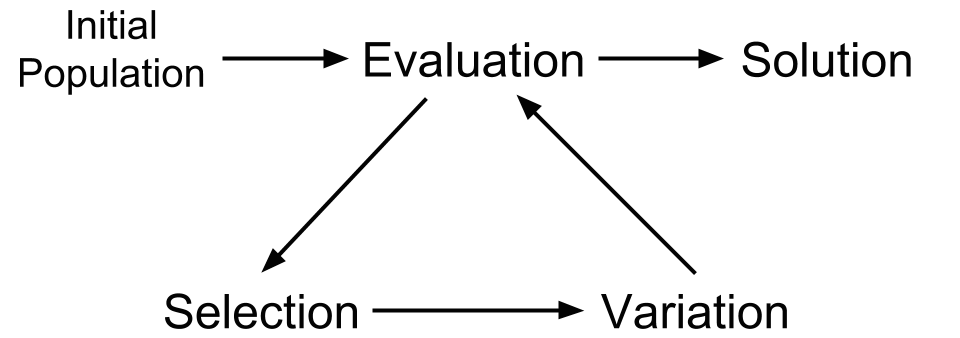
\includegraphics[width=0.25\textwidth]{res/EvolutionCycle}
\caption{Evolutionary Computation process.}
\label{fig:evo}
\end{figure}

Genetic Programming works by generating a initial population of random programs.  This population then follows the cycle in Figure \ref{fig:evo} until a solution is found or the run is considered a failure. To evaluate a program, it is given set of inputs and executed. The set of outputs produced by the program is compared with the desired outputs in order to produce a set of errors. 

This set of errors is used in the selection phase to pick programs whose performance merit them to be parents of the next generation of the population. This is done via a variety of selection algorithms, although it has been shown that lexicase selection generally leads to more solutions for IPS tasks~\cite{Helmuth2015a, Helmuth2015c, Forstenlechner:2017:eurogp}.

The selected parent programs are then recombined using a series of genetic operators in the variation phase of evolution. This results in a new generation of programs that share traits with their parent programs but are generally never identical.

After a program is produced that outputs the desired values on all input test cases, evolution is stopped and the program is tested on a entirely separate set of inputs to confirm generalization. If the program produces all correct outputs on the second set of inputs, it is considered a solution.

\subsubsection{PushGP}

Our first comparison genetic programming system, PushGP, evolves programs in a Turing complete, stack based language called Push~\cite{Spector2002, Spector2005}. Push features separate stacks for each data type, including code. Push programs are lists of instructions and literals. Literals are values that get placed on the stack corresponding to their type. Instructions are built-in functions that pop values off the stacks, modify them, and push them back on the appropriate stacks. Programs are run through an interpreter, which modifies the stacks. After all instructions and literals have been processed through the interpreter, the final state of the stacks is the output of the program.

PushGP was chosen as a comparison method because of its ability to evolve programs that can do the following:
\begin{itemize}
\item Manipulate all basic data types, including vectors.
\item Return multiple outputs.
\item Utilize iteration, recursion, conditional execution, and other more exotic control structures.
\end{itemize}

Given that the chosen problem set contains general software tasks that require all three of the above listed features, most commonly used Genetic Programming systems would be unable to adequately attempt to find a solution.

Implementations of PushGP systems are available in the Clojure programming language\footnote{https://github.com/lspector/Clojush}, as well as a new implementation in Python\footnote{https://github.com/erp12/Pysh}. The Basic Execution Models problems were run in the Python implementation of PushGP and the General Program Synthesis Benchmark Suite problems were run in the Clojure implementation. In both implementations, the instruction sets and genetic operators were identically implemented for this comparison.

\subsubsection{Grammar Guided Genetic Programming (G3P)}

The second genetic programming system used in this comparison is Grammar Guided Genetic Programming (G3P). It was recently shown by~\cite{Forstenlechner:2017:eurogp} that G3P can perform well on general IPS tasks if implemented in a particular way.

The G3P system described in~\cite{Forstenlechner:2017:eurogp} requires the specification of a Grammar and a Skeleton. 

The G3P system's grammar is composed of a separate context free grammar for each data type. Supported data types include: booleans, integers, floats, strings, lists of booleans, lists of integers, lists of floats, and lists of strings. There is also an addition grammar for the structure of the program.  These grammars are defined in Backus-Naur Form. Together these grammars form a single, general grammar that can be used to attempt arbitrary program synthesis tasks.

Aside from the grammar, the G3P system must be provided a skeleton. This skeleton contains the signature of the function that is going to be evolved. The signature specifies the inputs to the function and the return statement. In order to help avoid runtime errors, functions that implement protected operations (ie. division and logarithm) can also be included in the skeleton.

When an individual in the G3P system is to be evaluated, the code from the individual is placed into the function signature, thus creating a complete function that can be executed. The output of this function on the test cases is compared to the target outputs to receive an error vector.

As part of the G3P grammar definition, it is required to specify the number of variables usable by the system.~\cite{Forstenlechner:2017:eurogp} claims that 3 variables per data type is sufficient for all problems.

\section{Limitation of Comparison}

The problems described in section 3 were chosen to demonstrate a system's ability to perform general program synthesis tasks. Each system considered in the comparison is designed for different situations which resulted in a difficult comparison.

\subsection{Support For Multiple Outputs}

The benchmark problems we consider have different requirements on their outputs, including some problems that print outputs, some that functionally return outputs, and some that require multiple outputs. If a system does not support printing values, it was considered sufficient to return a single string containing all printed text, including newlines, in addition to the other output values.

Flash Fill only supports populating cells in a single column at once. The only way to produce multiple outputs using Flash Fill would be to generate each output value separately. Solving a problem in multiple parts was considered a fundamentally different IPS task, and thus a variety of problems were considered unable to be fully posed to Flash Fill.

MagicHaskeller also only supports synthesizing programs that produce a single output, however MagicHaskeller supports the tuple data type. Given that elements of a tuple do not have to be of the same data type, it was deemed adequate for MagicHaskeller to produce a single tuple containing all outputs for problems that required multiple outputs. For problems that called for printing values, one of the elements of the output tuple would be a string containing all printed text, including newlines.

The G3P grammars do not contain any methods of printing or formatting output values. Thus, any problems that required the use of printing or outputs given in a particular format (ie. A string with values printed on particular lines) must have been implemented in a way that did not require these behaviors. This implies that the G3P system was not posed the exact same IPS tasks, albeit very similar ones.

\subsection{Supported Data Types}

Many problems in the comparison required the handling of multiple data types, often including vectors.  Excel does not include a native vector or list data structure, and it is not clear what the best way to phrase problems that require vectors to Flash Fill. A string representation of vectors was attempted for some problems. If a problem specifies an input value will be a vector of fixed length, the problem can be posed with each element of the vector in its own cell. If the vector's length is not fixed, this cannot be done, because a tabular structure cannot be formed. If a problem requires a vector output, it cannot be posed to Flash Fill with elements in their own cell because generating each output value would be a separate IPS task. Due to this shortcoming of Flash Fill, there are a number of problems in this comparison that Flash Fill was unable to attempt.

G3P supports list types, but the supported list types contain values of a single data type. In other words, G3P can create and manipulate integer lists that can only contain integer values. There is no list type that can hold values of arbitrary types. This limitation, combined with the previous mentioned lack of printing methods, resulted in no adequate G3P implementation of the "String Differences" problem.

\subsection{Number of Training and Test Cases}

The number of nested predicates that can be given to MagicHaskeller is very limited, and if too many predicates are given the system will produce memory errors. This is a consequence of MagicHaskeller being a web hosted service where resources are shared between all users. Due to this limitation, it was not possible to give MagicHaskeller the same training dataset as the other IPS methods. Although this weakens the presented results, it speaks to the usability and flexibility of the web hosted MagicHaskeller system.

\subsection{Access To Systems}

There is not publicly available implementation of TerpreT, and thus it is only known how TerpreT performs on the \emph{Basic Execution Models} problem set. It is unknown how TerpreT would perform on the \emph{General Program Synthesis Benchmark Suite}.

Given how recently the G3P system for general program synthesis was presented, it has not been applied to the \emph{Basic Execution Models} problem set. These results would be informative and likely be fairly easy to obtain.

Flash Fill is not open-source, which makes it impossible to modify for new tasks.

\section{Results}

\begin{figure}
\begin{tabular}{ r | c c c c }
	& TerpreT & Flash Fill & MH & PushGP \\
	\hline
	Invert & \checkmark & $x$ & \checkmark & \checkmark \\
	Prepend Zero & \checkmark & \checkmark & \checkmark & \checkmark \\
	Binary Decrement & \checkmark & $x$ & $x$ & $x$ \\
	2BCSR & \checkmark &  & $x$ & \checkmark \\
	Full Adder & \checkmark &  & $x$ & \checkmark \\
	2 Bit Adder & \checkmark &  & x & $x$ \\
	Access & \checkmark & $x$ & \checkmark & \checkmark \\
	Decrement & \checkmark & $x$ & \checkmark & \checkmark \\
\end{tabular}
\caption{Results of applying TerpreT, Flash Fill, MagicHaskeller (MH) and PushGP on the Basic Execution Models problems from~\cite{Gaunt2016}.  A check denotes the system could find a solution. An $x$ denotes the problem was fully posed to the system, but a solution was not found. No symbol denotes the problem could not be fully posed to the system.}
\label{fig:results1}
\end{figure}

\begin{figure}
\begin{tabular}{ r | c c c c }
	& Flash Fill & MH & PushGP & G3P \\
	\hline
	Number IO & $x$ & \checkmark & \checkmark & \checkmark \\
	Small Or Large & $x$ & $x$ & \checkmark & \checkmark \\
	For Loop Index & $x$ & $x$ & \checkmark & \checkmark \\
	Compare String Lengths & $x$ & $x$ & \checkmark & \checkmark \\
	Double Letters & $x$ & $x$ & \checkmark & $x$ \\
	Collatz Numbers & $x$ & $x$ & $x$ \\
	Replace Space with Newline &   & $x$ & \checkmark & $x$ \\
	String Differences & $x$ & $x$ & $x$ \\
	Even Squares & $x$ & $x$ & \checkmark & \checkmark \\
	Wallis Pi & $x$ & $x$ & $x$ \\
	String Lengths Backwards &   & \checkmark  & \checkmark & \checkmark \\
	Last Index of Zero &  & $x$ & \checkmark & \checkmark \\
	Vector Average &  & \checkmark & \checkmark & $x$ \\
	Count Odds &  & $x$ & \checkmark & \checkmark \\
	Mirror Image &  & $x$ & \checkmark & \checkmark \\
	Super Anagrams & $x$ & $x$ & $x$ & \checkmark \\
	Sum of Squares & $x$ & $x$ & \checkmark & \checkmark \\
	Vectors Summed &  & \checkmark & \checkmark & \checkmark \\
	X-Word Lines & $x$ & $x$ & \checkmark & x \\
	Pig Latin & $x$ & $x$ & $x$  \\
	Negative To Zero &  & \checkmark & \checkmark & \checkmark \\
	Scrabble Score & $x$ & $x$ & \checkmark & $x$ \\
	Word Stats & $x$ & $x$ & $x$ \\
	Checksum & $x$ & $x$ & \checkmark \\
	Digits & $x$ & $x$ & \checkmark & $x$ \\
	Grade & $x$ & $x$ & \checkmark & \checkmark  \\
	Median & $x$ & $x$ & \checkmark & \checkmark \\
	Smallest & $x$ & \checkmark & \checkmark & \checkmark \\
	Syllables & $x$ & $x$ & \checkmark & $x$ \\
\end{tabular}
\caption{Results of Flash Fill, Magic Haskeller (MH), PushGP, and Grammar Guided Genetic Programming (G3P0) on the Software Synthesis Benchmark Suite from~\cite{Helmuth2015b}. A check denotes the system could find a solution. An $x$ denotes the problem was fully posed to the system, but a solution was not found. No symbol denotes the problem could not be fully posed to the system. When the original benchmark paper~\cite{Helmuth2015b} was published, PushGP had not been able to find solutions to the Checksum problem. Subsequent unpublished work found that expanding the set of test cases led to the discovery of solutions.}
\label{fig:results2}
\end{figure}

Although inductive program synthesis is often thought of as a single field, it is clear from this comparison that IPS methods are generally implemented with a narrow domain in mind. This is made most evident by the limitations discussed in section 4. After making strong efforts to overcome these limitations, the results of applying each IPS method to the problem sets described in section 2 were compiled into Figure \ref{fig:results1} and Figure \ref{fig:results2}.

Flash Fill performed particularly poorly on the the considered problems. Being designed for string manipulation, it is not surprising that it can only solve the "Prepend Zero" problem, where the input binary string is implemented as a text string of $1$s and $0$s. On all other problems, Flash Fill does not produce a solution. This is not unexpected because no other problem is solely comprised of such simple text manipulation.

MagicHaskeller was only able to solve 10 out of the 37 problems it was applied to. These problems tended to mainly involve applying simple operations to each element of a vector, or simple forms of aggregation.

% Terpret Problems
The system that performed the best on the \emph{Basic Execution Models} problems was TerpreT, while PushGP failed to solve 2 of the 8 problems. Given the success of TerpreT in this domain, it would be interesting to know how the system performs on the \emph{Software Synthesis Benchmark Suite}. The only system for which there is no results on the \emph{Basic Execution Models} problems is G3P. These results would be very informative and relatively simple to obtain. Given how recently this specific G3P technique was posed these results have not been gathered yet.

% Software Benchmark Problems
Both genetic programming systems clearly outperformed Flash Fill and MagicHaskeller on the \emph{Software Synthesis Benchmark Suite}. PushGP solved  23 out of the 29 problems, and G3P solved 16 of the 29 problems.

% Runtime and deterministic/stocastic
It must be mentioned that there is an enormous difference in runtime and computation power required for these IPS systems. FlashFill and MagicHaskeller produce an output, or report failure, in near instantaneous time. TerpreT, PushGP  and G3P require many hours to complete a single run and due to their stochastic nature, often require many runs. It is not entirely uncommon to spend weeks of CPU time on multiple PushGP runs of a single problem and only encounter a small number of solutions, meanwhile MagicHaskeller can produce the same solution every time, nearly instantaneously. 

% Output readability
Some of the considered IPS methods were designed with other functionality in mind, aside from solving IPS task. For example, MagicHaskeller, G3P, and TerpreT produce readable source code. PushGP produces code in the Push language, but it cannot be used outside of a Push interpreter and is not easily read by humans. FlashFill does not provide any access to the solution program.

\begin{figure}
\begin{tabular}{ r | l }
\textbf{Problem} & \textbf{Solution} \\
\hline
Invert & \texttt{f = (map (\textbackslash b -> abs(b -1 )))} \\
Decrement & \texttt{f = (map (subtract 1))} \\ 
String Lengths Backwards & \texttt{f = (\textbackslash a -> reverse (map length a))} \\
Negative To Zero & \texttt{f = (map (\textbackslash b -> max b 0)} \\
\end{tabular}
\caption{Some example solutions produced by MagicHaskeller.}
\label{fig:MHsolutions}
\end{figure}

Example source code produced by MagicHaskeller is shown in in Figure \ref{fig:MHsolutions}.

\section{Conclusion}

This paper attempts to compare the TerpreT, PushGP, G3P, Flash Fill and MagicHaskeller inductive program sythesis systems. The comparison was carried out using problem sets that requires producing programs in low level domains, such as boolean logic, as well as high level domains that require the synthesis of programs similar to what humans write.

The recently unveild TerpreT system shows effectiveness in low level domains, but there are results to suggest it can perform well on different kinds of problems. FlashFill performs quickly and adequately on some simple string manipulation task as designed, but did not show any capabilities of operating outside this narrow domain.MagicHaskeller is very capable of performing list comprehensions and certain other simple tasks, but consistently fails to solve problems that require a large number of training instances. PushGP continues to do reasonably well across a broad range of problems, but can be quite expensive when compared to Flash Fill and MagicHaskeller. Grammar Guided Genetic Programming has the added functionality over PushGP of producing usable source code in any language, while still finding solutions to almost as many problems.

The most conclusive finding that has come out of this comparison is that not all IPS systems can be applied to the same problems. This makes comparison extremely difficult. As access to open source implementations of these systems become more available, it will be easier to extend them to allow for more supported data types, and other features that make comparison easier.

It is very clear that certain IPS systems are not suited for some applications depending on if runtime and computational power are concerns. It does appear that the genetic programming methods, although being significantly more computationally expensive, are designed to be more flexible in regards to the types of problems they can be applied to.

